 \section{Durchführung}
\label{sec:Durchführung}

Die in der Theorie und im Folgenden vorgestellten Schaltungen werden für die Modulation und
Demodulation amplituden- und frequenzmodulierter Schwingungen benutzt.

\begin{figure}[H]
  \centering
  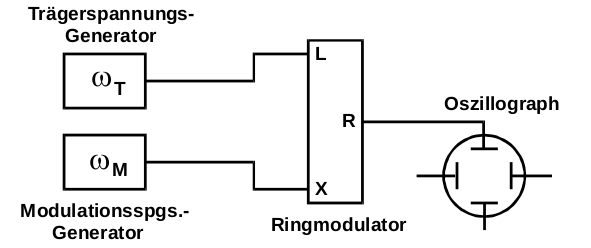
\includegraphics[height=3.4cm]{JasperErsterSchultag/expab.png}
  \caption{Schaltung zur Erzeugung einer amplitudenmodulierten Schwingung mit Hilfe eines Ringmodulators \cite{anleitung}.
  Das Oszilloskop kann je nach Messung beispielsweise durch einen Frequenzanalysator ausgetauscht werden.}
  \label{fig:expab}
\end{figure}

\begin{figure}[H]
  \centering
  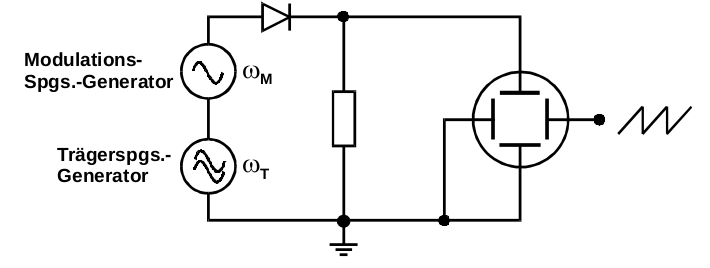
\includegraphics[height=3.7cm]{JasperErsterSchultag/expc.png}
  \caption{Schaltung zur Erzeugung einer amplitudenmodulierten Spannung mit Hilfe einer Diode \cite{anleitung}.}
  \label{fig:expc}
\end{figure}

\begin{figure}[H]
  \centering
  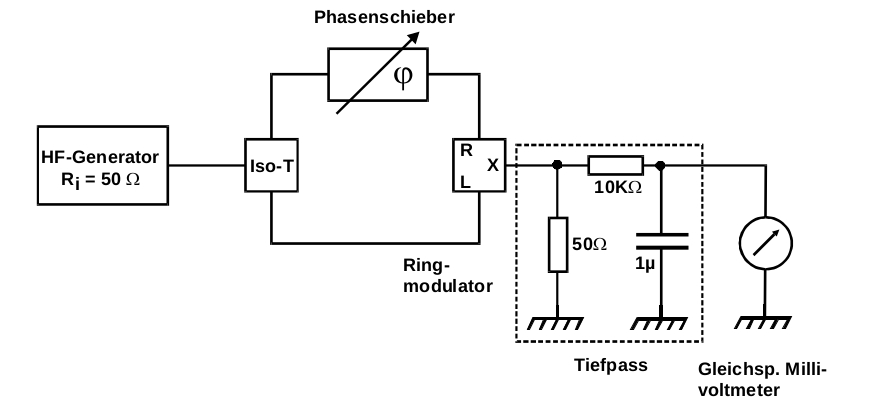
\includegraphics[height=5.3cm]{JasperErsterSchultag/expef.png}
  \caption{Schaltung zur Überprüfung, ob sich der Ringmodulator auch zur Demodulation als
  phasenempfindlicher Gleitrichter eignet \cite{anleitung}.}
  \label{fig:expef}
\end{figure}

Es werden folgende Experimente durchgeführt:
\begin{enumerate}
  \item Im ersten Teil wird mit Hilfe der Schaltung aus Abbildung \ref{fig:expab} eine
  amplitudenmodulierte Schwingung mittels eines Ringmodulators erzeugt. Es wird ein
  Bild der entstehenden Schwebung und außerdem Modulations- und Trägerfrequenz und -spannung
  aufgenommen.
  \item Als nächstes wird anstatt des Oszilloskops ein Frequenzanalysator in die Schaltung eingebaut
  und so das Frequenzspektrum der modulierten Schwingung aufgenommen.
  \item Im nächsten Schritt wird mit Hilfe der Schaltung aus Abbildung \ref{fig:expc} eine amplitudenmodulierte Schwingung
  mittels einer Diode erzeugt. Erneut wird ein Bild der entstehenden Schwebung, Modulations- und Trägerfrequenz und -spannung und
  das Frequenzspektrum aufgenommen.
  \item In diesem Teil der Durchführung wird eine frequenzmodulierte Schwingung mit der Schaltung aus Abbildung \ref{fig:freqmodschaltung}
  erzeugt. Ab einer Modulationsfrequenz von etwa $\SI{1}{\kilo\hertz}$ ist eine Verschmierung der modulierten Wechselspannung hervorgerufen
  durch Phasenverschiebung gemäß Abschnitt \ref{sec:bestmod} erkennbar. Ein Bild von dieser Verschmierung und außerdem das Frequenzspektrum
  der modulierten Schwingung werden aufgenommen.
  \item Als nächstes wird versucht, mit Hilfe der Schaltung aus Abbildung \ref{fig:expef} zu zeigen, dass der Ringmodulator
  auch zur Demodulation verwendet werden kann. Dafür wird die Proportionalität der am Ausgang X anliegenden Spannung zum
  Kosinus der Phase $\varphi$ zwischen den Wechselspannungen an den Eingängen L und R überprüft.
  \item Nun wird mit dem Ringmodulator gemäß Abbildung \ref{fig:ampldemodschaltung1} eine amplitudenmodulierte Schwingung
  demoduliert. Es wird ein Bild mit dem Oszilloskop aufgenommen, an dem sowohl die Eingangsmodulationsspannung, als auch die
  modulierte und demodulierte Modulationsspannung verglichen werden.
  \item Im nächsten Schritt wird eine amplitudenmodulierte Schwingung mit Hilfe einer Diode gemäß Abbildung \ref{fig:ampldemodschaltung2}
  demoduliert. Sowohl an der Stelle A, als auch nach dem Tiefpass wird ein Bild aufgenommen, an welchem die Eingangsmodulationsspannung und
  die modulierte und demodulierte Modulationsspannung vergleichbar sind.
  \item Im letzten Schritt wird versucht, eine frequenzmodulierte Schwingung mittels Schaltung \ref{fig:flankendemodulator} zu demodulieren.
  Es wird ein Bild am Oszilloskop nach dem Schwingkreis, an dem die frequenzmodulierte Schwingung zu einer amplitudenmodulierten umgewandelt
  wurde, nach der Diode, an welcher ein Vorzeichen der Spannung abgeschnitten wird, und nach dem Tiefpass, an dem die Modulationsfrequenz
  herausgefiltert wird, aufgenommen. ABSÄTZE !!!!!!!!!!!!!
\end{enumerate}
